\documentclass[11pt]{article}
\usepackage[margin=1in]{geometry}
\usepackage[T1]{fontenc}
\usepackage{amsmath,amssymb,booktabs,graphicx,hyperref,xcolor,array,caption,colortbl,multirow,algorithm,algorithmic}
\usepackage[numbers,sort&compress]{natbib}
\captionsetup{font=small,labelfont=bf}
\newcommand{\todo}[1]{{\color{red}[\textbf{TODO:} #1]}}
\newcommand{\cn}[1]{{\color{orange}[\textbf{CITATION NEEDED:} #1]}}
\newcommand{\verify}[1]{{\color{blue}[\textbf{VERIFY:} #1]}}
\newcommand{\fake}[1]{{\color{red}#1}}            % PLACEHOLDER: số liệu/thông tin giả, thay trước khi nộp (xem paper/PLACEHOLDERS.md)
\newcommand{\best}[1]{\cellcolor{gray!20}\textbf{#1}}

\title{How Far Can Simulation Take Root Cause Diagnosis in Milling?\\
Provenance-Tracked Simulation, Real-Data Gap Measurement and the Circularity of Simulated RCA Benchmarks}
\author{Hai-Dang Dang$^{1}$ \and Dinh Thieu Quang$^{1}$ \and Simon Park$^{1,*}$\\[3pt]
{\normalsize $^{1}$VinUniversity, Hanoi, Vietnam}\\[2pt]
{\normalsize \fake{hai-dang.dang@vinuni.edu.vn \quad dinh.quang@vinuni.edu.vn \quad $^{*}$simon.park@vinuni.edu.vn}}}   % PLACEHOLDER emails
\date{\textbf{DRAFT v3} --- target venue: IEEE CASE 2027 (deadline 1 March 2027; format not yet converted).\\
{\color{red}Red text marks placeholders (author e-mails, archival DOI, and all values in the planned real-data evaluation); they are not results.}}

\begin{document}
\maketitle

\begin{abstract}
Diagnosing the root cause of a machining fault (loose fixture, worn tool, excessive depth, unsuitable spindle speed) is attractive to learn from simulated data, because real cuts with known causes are scarce.
Whether simulation actually supports such diagnosis is rarely measured: simulated benchmarks usually build the diagnostic nodes from the same generator that produces the test faults, and the gap to real signals is not quantified component by component.
We therefore treat simulation-based diagnosis as a measurement problem.
We build a regenerative-milling simulator in which every parameter is tagged as fixed, ranged, learned or assumed, ground its healthy baseline in real multi-sensor spectra, and compare it with real data along three axes: healthy baseline, fault signature, and transfer to unseen machines.
In a causal root-cause-ranking benchmark, top-1 accuracy at ten anomalous samples is 0.80--0.98 for five of six algorithms when nodes and faults share a generator, but 0.35--0.71 when the generator's physical parameters are shifted at test time (0.32--0.62 with a stiffer, stable-regime parameter set); replacing the causal graph by a shuffled or empty one changes nothing, and label-free nodes give near-chance accuracy, so the benchmark measures supervised node estimation, not causal reasoning.
The simulated healthy baseline remains distinguishable from real data (balanced accuracy $0.82\pm0.04$), neither the simulated faults nor a once-per-revolution chipped-flute mechanism reproduces the low-frequency, tonal signature of a real defective tool, and at nominal parameters the simulator lies above its own stability limit for every real cutting condition, so fault effects must be rescaled by gains of order $10^{-5}$.
On a public three-machine wear dataset, a model trained only on simulated wear and applied to unseen machines without real labels reaches wear-detection AUROC 0.89, 0.81 and 0.57, which is below a one-feature force-RMS rule on two of the three machines (0.99, 0.99, 0.46), and fine-tuning it with real labels is no better than training from scratch (at earlier-wear thresholds it is higher than the rule on average, but only because of one machine); domain-adaptation baselines add nothing over gradient boosting on this task.
Transfer to unseen machine--tool combinations does not degrade with a spectral proxy for dynamics distance (nine targets), so these data cannot test whether simulation is needed to extrapolate to new dynamics.
We conclude that this wear task is too easy to show a benefit of simulation, that benchmark design can inflate apparent diagnostic accuracy, and we release the protocol and code to test these conclusions on harder, real multi-cause data.
\end{abstract}

%% =============================================================================================
\section{Introduction}
Machine-tool operators and process engineers need to know \emph{why} a milling operation misbehaves, not only \emph{that} it does, because the remedy differs: re-clamp the part, change the tool, reduce the depth or move the spindle speed.
Public machining datasets record sensor streams and, at best, expert labels of normal or abnormal operation; ground-truth root causes are rare \citep{kim2026msm}.
Simulation is the obvious substitute, and training on simulated data and applying it to a real machine has been shown to work for chatter detection \citep{alberts2024sim2real} and tool-fault monitoring \citep{ebrahimi2023smartfaults}.
Both studies, however, consider a single fault family on one machine, and neither asks how much of the reported accuracy comes from the simulator itself.

\begin{figure}[t]\centering
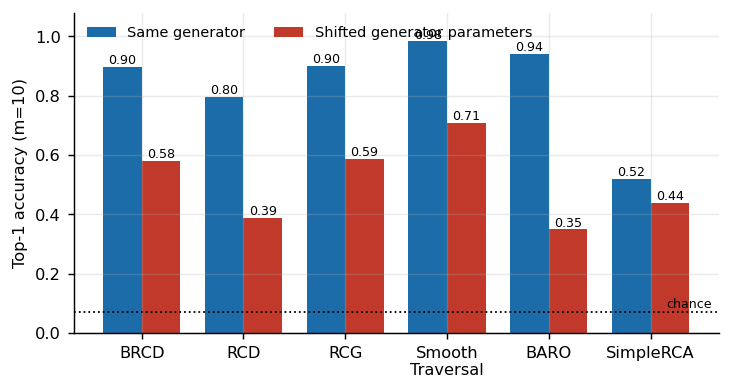
\includegraphics[width=0.72\linewidth]{figures/f_teaser.png}
\caption{Teaser: top-1 root-cause accuracy of six causal RCA algorithms (mean over five root causes, $m{=}10$ anomalous samples; dotted line: chance) when the diagnostic nodes and the test faults come from the same simulator (blue) and when the simulator's physical parameters are shifted at test time (red).}\label{fig:teaser}
\end{figure}

\paragraph{The unresolved problem.}
For root cause analysis, the gap between a simulated benchmark and real diagnosis has three separate parts that existing work does not separate: (i) the healthy baseline of the simulator may differ from real signals; (ii) the simulated fault signatures may differ from real ones; and (iii) the diagnostic procedure may exploit the generator, for example when the nodes of a causal graph are trained on labels produced by the same simulator that generates the test faults.
Without separating them, a high simulated accuracy cannot be interpreted (Figure~\ref{fig:teaser}).

\paragraph{Our approach.}
We build a simulator whose parameters carry their provenance and measure each part of the gap against real data (Figure~\ref{fig:pipeline}).
The healthy baseline is modelled from real spectra rather than simulated, so that part (i) can be tested directly; fault signatures are compared with a real defective tool for part (ii); and part (iii) is tested by shifting the generator's parameters at test time and by ablating the graph and the node construction.

\begin{figure}[t]\centering
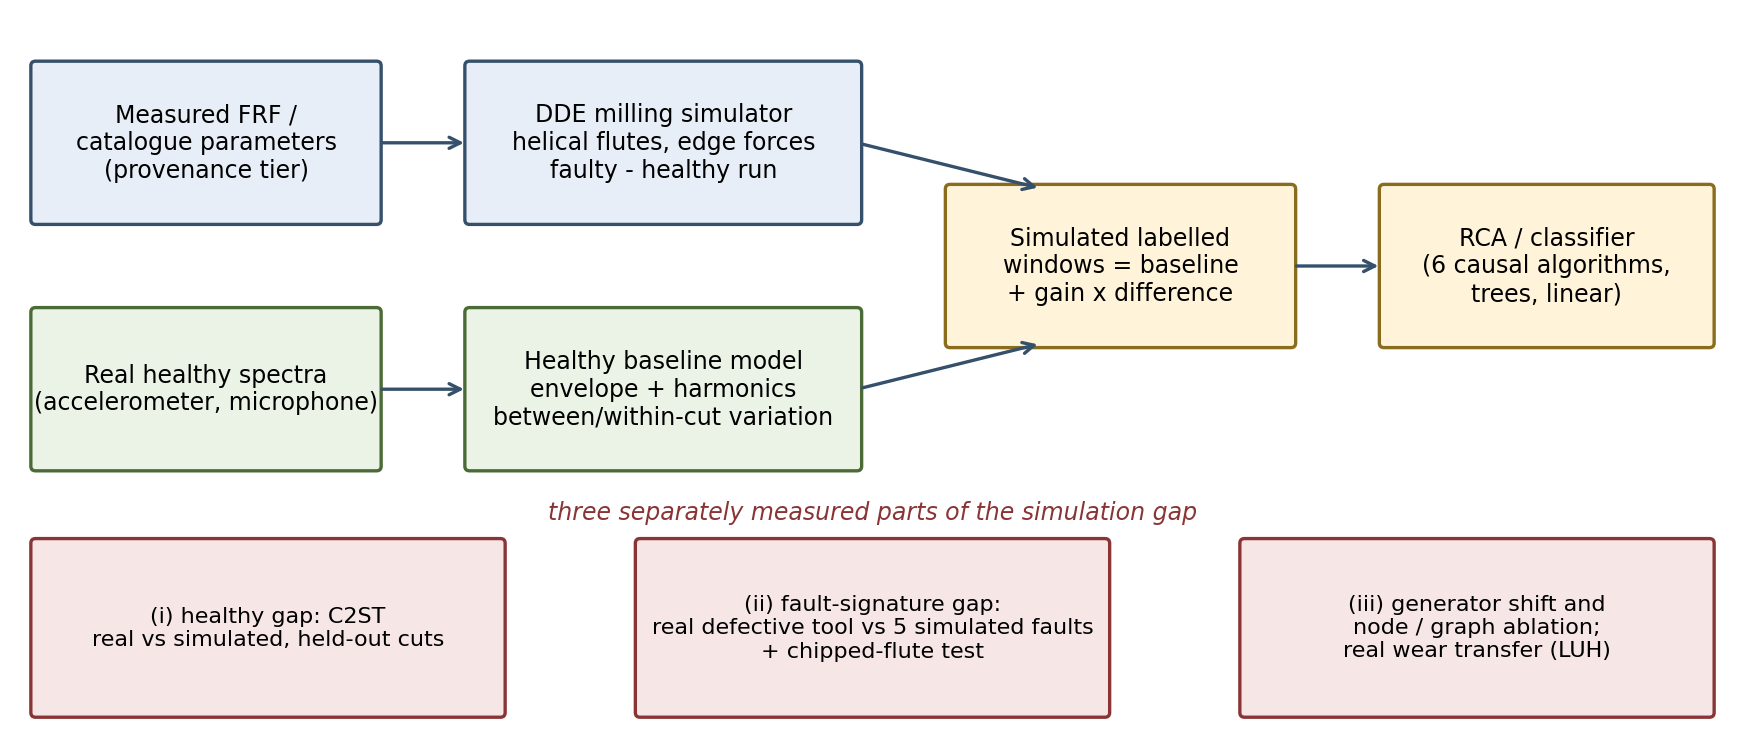
\includegraphics[width=0.97\linewidth]{figures/pipeline.png}
\caption{Overview. The simulator supplies fault \emph{differences} only; the healthy baseline comes from real data; each part of the simulation gap is tested separately.}\label{fig:pipeline}
\end{figure}

\paragraph{Contributions.}
\begin{enumerate}
\item \textbf{A measurement of benchmark circularity.} Top-1 accuracy of six causal RCA algorithms falls from 0.80--0.98 to 0.35--0.71 under moderate parameter shift, the causal graph carries no information in the benchmark, and the result is decided by how nodes are constructed (Section~\ref{sec:circ}).
\item \textbf{A component-wise gap measurement with negative results.} A real-data baseline and a classifier two-sample test quantify the healthy gap; a real defective tool shows that low-frequency and tonal components are not reproduced by any simulated fault, including a chipped-flute mechanism; and a stability analysis shows that the nominal simulator operates above its stability limit (Sections~\ref{sec:regime}, \ref{sec:healthy}, \ref{sec:real}).
\item \textbf{Evidence on when simulation helps on real data.} On a public multi-machine wear dataset, simulation-only transfer is machine-dependent and below a one-feature baseline, fine-tuning gives no benefit, and domain-adaptation baselines add nothing, so the task cannot show a benefit of simulation (Section~\ref{sec:wear}).
\item \textbf{A parameter-provenance policy, an open simulator with FRF import, a detailed account of the RCA algorithms as implemented (including their deviations from the originals), and an evaluation protocol} to be run on real multi-cause data (Sections~\ref{sec:sim}, \ref{sec:rca}, \ref{sec:limits}).
\end{enumerate}

\paragraph{What we do not show.}
We have no validation of root-cause \emph{ranking} on real multi-cause data. Simulation remains the only practical source of labelled data for causes that cannot be collected in numbers, so we do not argue that it is unnecessary; we show that its fidelity is not yet established and that, on the real data we could test, it was not needed. Whether it is needed for causes without real labels, or for machines outside the training dynamics, is the question the protocol of Section~\ref{sec:limits} is designed to answer.

%% =============================================================================================
\section{Related Work}
\paragraph{Simulation-trained diagnosis in machining.}
\citet{alberts2024sim2real} train a random forest on more than 140\,000 simulated chatter cases, then fine-tune it with 10\% of 1\,600 real instances from one custom 3-axis machine to reach 86.1\% accuracy on a chatter-versus-stable decision.
\citet{ebrahimi2023smartfaults} train random forests on analytical process-simulation data to monitor tool-related faults in milling and report 94\% accuracy, and 93\% on actual measurements (from the abstract; full text not read), and \citet{yesilli2022tlchatter} transfer chatter detectors between conditions.
These works establish that simulation-to-real training is feasible for one fault family on one machine; they do not address several root causes, a change of machine, or the share of accuracy attributable to the generator (Table~\ref{tab:related}).

\begin{table}[t]\centering\footnotesize
\caption{Comparison with the closest prior work. ``--'' means not addressed or not stated.}\label{tab:related}
\begin{tabular}{p{2.1cm}p{2.5cm}p{2.5cm}p{2.9cm}p{2.9cm}}\toprule
Work & Domain and task & Real data & Role of simulation & Tests generator dependence\\\midrule
\citet{alberts2024sim2real} & milling; chatter vs.\ stable (one fault family) & one custom 3-axis machine, MEMS sensor; 1\,600 instances & random forest trained on $>$140\,000 simulations, fine-tuned on 10\% real & limitations stated; no systematic test\\
\citet{ebrahimi2023smartfaults}$^{\ddagger}$ & milling; tool-related faults (types not stated in the abstract) & actual measurements (93\% reported) & random forest trained on analytical simulation data (94\% reported) & --\\
\citet{yesilli2022tlchatter}$^{\ddagger}$ & chatter detection across conditions & experimental & transfer between conditions & --\\
\citet{lee2026brcd} & causal RCA, cloud microservices (not machining) & three microservice systems & synthetic benchmarks for the algorithm & compares 10 RCA methods; notes marginal-deviation baselines (BARO, SimpleRCA) are strong on two systems\\
\textbf{This work} & milling; five root causes, wear detection & MSM (73 cuts), defective tool, LUH (3 machines) & provenance-tagged simulator; fault differences added to a real-data baseline & shared vs.\ shifted generator; graph and node ablations; real-signature comparison\\\bottomrule
\end{tabular}\\[2pt]
{\footnotesize $^{\ddagger}$ from title and abstract only; full text not read.}
\end{table}

\paragraph{Transfer across machines and conditions for tool wear.}
Domain-adversarial transfer \citep{wang2020datwear}, meta domain generalisation \citep{li2023metadg} and physics-guided or hybrid models \citep{li2025physguided,yang2022hybridwear} address changes of cutting condition or machine for wear, using real data of the source domains. We use DANN-style and CORAL-style adaptation as baselines on the public wear data (Section~\ref{sec:wear}); meta domain generalisation is left for the real multi-cause data.

\paragraph{Causal root cause analysis.}
RCD \citep{ikram2022rcd} localises root causes with conditional-independence tests against a failure indicator, RCG \citep{ikram2025rcg} ranks candidates by conditional mutual information given the parents in a partial causal structure, BARO \citep{pham2024baro} uses Bayesian change-point detection and a robust deviation score, SimpleRCA \citep{fang2025simplerca} compares the maximum of the anomalous data with the 95th percentile of the normal data, and Smooth Traversal \citep{orchard2025} traverses ancestors of a trigger node using outlier scores. BRCD \citep{lee2026brcd} computes a Bayesian posterior over root causes from a CPDAG learned before the failure, with consistency guarantees. These methods were developed and evaluated for software systems; \citet{lee2026brcd} themselves observe that methods based on the marginal deviation of the anomalous data (BARO, SimpleRCA) are competitive on some systems but do not generalise. Our finding that the graph is irrelevant in the machining benchmark is consistent with, and a more extreme case of, that observation. Applying these algorithms to machining needs a source of faults with known causes, which is the role of simulation here. Importantly, the algorithms in our code base are simplified re-implementations on a known graph, not the authors' code (Section~\ref{sec:rca}).

\paragraph{Calibrating simulators to data.}
Calibration with a discrepancy term \citep{kennedy2001}, domain randomisation \citep{tobin2017}, adversarial refinement \citep{shrivastava2017} and simulation-based inference \citep{cranmer2020} are the standard tools. We use a classifier two-sample test as a diagnostic, not as a training signal \citep{lopezpaz2017c2st}.

%% =============================================================================================
\section{Study Design and Data}\label{sec:data}
We use three real sources, each for one question (Table~\ref{tab:data}).
\begin{table}[t]\centering\small
\caption{Real data used and the question each answers.}\label{tab:data}
\begin{tabular}{p{3.2cm}p{5.8cm}p{5.2cm}}\toprule
Source & Content used & Question\\\midrule
MSM, machine \texttt{imi\_vm20i}, datasets 5, 6 \citep{kim2026msm} & 73 cuts (48 normal, 25 abnormal), 2-flute 6.35~mm tool, AA~6061 (wet), 9000--12000~rpm, three radial depths, 219 windows of 0.3~s & Healthy baseline and gain calibration (Sec.~\ref{sec:base})\\
MSM datasets 3 and 14 & Intentionally defective 12.7~mm four-flute tool D$^*$ (12 cuts) and healthy tool (64 cuts), AISI 4140 & Fault signature (Sec.~\ref{sec:real})\\
LUH \citep{denkena2023luh} & Three machines $\times$ three tools, 406 runs, force at 25~kHz, flank wear VB & Cross-machine transfer and sim-to-real wear (Sec.~\ref{sec:wear})\\\bottomrule
\end{tabular}
\end{table}
In datasets 5 and 6 the abnormal label is strongly associated with up-milling (all 36 down-milling cuts are normal), so it is not a specific root cause. Spindle speed and feed in the label files equal the controller-recorded values (ratio 1.000).

%% =============================================================================================
\section{The Simulator}\label{sec:sim}
\subsection{Overview}
Given a cutting condition, the framework produces labelled simulated windows in three steps: a delay-differential-equation (DDE) simulator provides the effect of a fault as a \emph{difference} between a faulty and a healthy run (this section); a baseline model fitted to real spectra provides the healthy signal (Section~\ref{sec:base}); and the scaled difference is added to the baseline (Section~\ref{sec:fault}). Section~\ref{sec:rca} defines the RCA methods that consume these windows.

\subsection{Structural dynamics and cutting forces}
\paragraph{Motivation.} Regenerative chatter arises from the delayed feedback between the vibration marks left by one tooth and the chip thickness of the next; a time-domain model with the correct delay captures both stable forced vibration and saturated chatter.
\paragraph{Design.} Each tool-tip axis $q\in\{x,y\}$ is a sum of modes with transfer function
\begin{equation}
H_q(s)=\sum_{r}\frac{\beta_r s+\alpha_r}{s^2+2\zeta_r\omega_r s+\omega_r^2},\qquad \beta_r=2\sigma_r,\;\;\alpha_r=2(\zeta_r\omega_r\sigma_r-\omega_{d,r}\nu_r),
\end{equation}
(residues $\sigma_r,\nu_r$; the nominal tool uses one mode per axis with $H=1/[m(s^2+2\zeta\omega s+\omega^2)]$, $m=k/\omega^2$). Each mode is a two-state system $[x_r,\dot x_r]$ discretised exactly with a zero-order hold, $(A_d,B_d)$ read from the matrix exponential of $\bigl(\begin{smallmatrix}A\,\Delta t & B\,\Delta t\\ 0&0\end{smallmatrix}\bigr)$, at $\Delta t=1/25\,600$~s.
Tooth $k$ of a flute with $N$ teeth is divided into $N_z{=}8$ axial slices of height $dz=a/N_z$; the angle of slice $q$ at time $t$ is
\begin{equation}
\phi_{k,q}(t)=\Omega t+\frac{2\pi k}{N}-z_q\frac{2\tan\beta}{D},\qquad z_q=(q+\tfrac12)dz,
\end{equation}
where $\Omega$ is the spindle angular speed, $\beta$ the helix angle and $D$ the tool diameter. A slice cuts only while $\phi_{k,q}\in[\phi_{st},\phi_{ex})$, with span $\arccos(1-2a_e/D)$ (up milling: $[0,\text{span})$; down milling: $[\pi-\text{span},\pi)$). Its chip thickness depends on the current and delayed displacement,
\begin{equation}
h_{k,q}=\Big[f_t\sin\phi_{k,q}+\big(x(t)-x(t-T)\big)\sin\phi_{k,q}+\big(y(t)-y(t-T)\big)\cos\phi_{k,q}+\nu_k(t)\Big]_{0}^{h_{\max}},\quad T=\frac{60}{N\,n},
\end{equation}
with $n$ the spindle speed in rpm, $f_t$ the feed per tooth (offset by $\pm$ the runout for the first two teeth), a fractional delay $T/\Delta t$ implemented by linear interpolation, tooth-wise roughness noise $\nu_k\sim\mathcal N(0,0.02\,\mu\text{m})$, and $h_{\max}=0.3$~mm. The elemental forces are
\begin{align}
dF_t&=(K_t h+K_{te})\,dz,\qquad dF_r=(K_rK_t h+K_{re})\,dz,\\
F_x&\mathrel{+}=-dF_t\cos\phi-dF_r\sin\phi,\qquad F_y\mathrel{+}=dF_t\sin\phi-dF_r\cos\phi,
\end{align}
and spindle imbalance $U$ adds $U\Omega^2[\cos\Omega t,\sin\Omega t]$. The helix angle is $\beta=30^\circ$ (manufacturer series feature list; medium confidence).
\paragraph{Stability lobes.} For comparison the zero-order approximation \citep{altintas2020} gives, for each chatter frequency $\omega_c$, the eigenvalue $\Lambda=-\frac{1}{2a_0}\big(a_1-\sqrt{a_1^2-4a_0}\big)$ with $a_0=H_xH_y(\alpha_{xx}\alpha_{yy}-\alpha_{xy}\alpha_{yx})$ and $a_1=\alpha_{xx}H_x+\alpha_{yy}H_y$, the limit depth $a_{\lim}=-\frac{2\pi\Lambda_R}{NK_t}(1+\kappa^2)$, $\kappa=\Lambda_I/\Lambda_R$, and the spindle speeds $n=60/(N T_k)$, $T_k=(\pi-2\psi+2k\pi)/\omega_c$, $\psi=\arctan(\Lambda_I/\Lambda_R)$.
\paragraph{Advantage and check.} Because the delay and the time-varying force direction are explicit, the same code reproduces forced vibration, saturated chatter and the effect of a stiffness, damping, force or speed change. With helix and edge forces off, the numba core reproduces a pure-Python straight-flute reference to $7\times10^{-16}$, eight slices are converged, and a time-domain grid agrees with the zero-order lobe prediction on 79\% of speed--depth points, with disagreement at moderate depth where the zero-order approximation is known to be conservative (Figure~\ref{fig:lobes}).

\begin{figure}[t]\centering
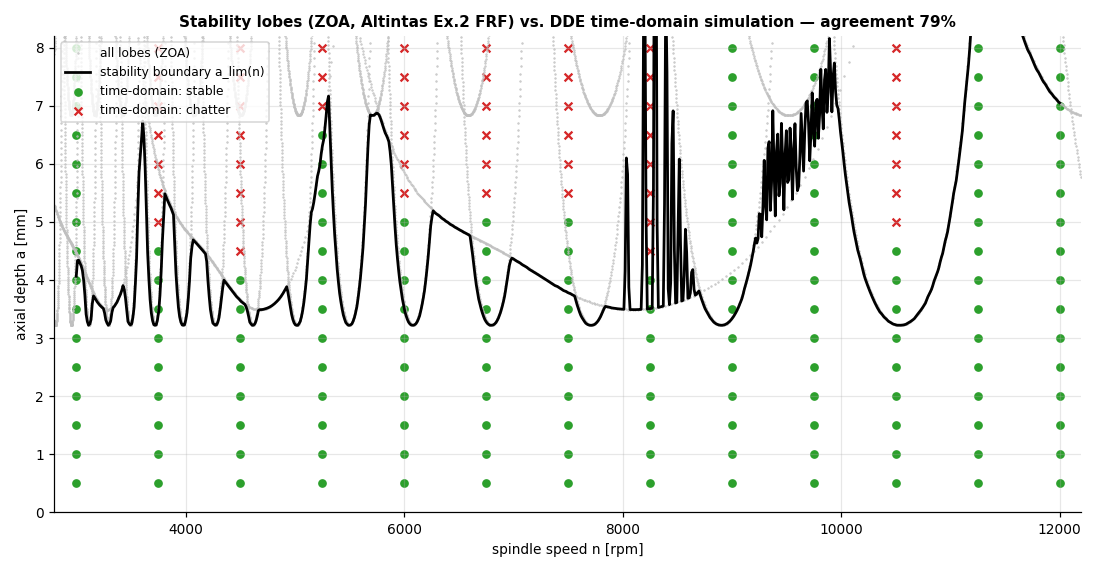
\includegraphics[width=0.72\linewidth]{figures/exp1_lobes_validation.png}
\caption{Stability lobes (zero-order approximation, 4-flute reference transfer function) and time-domain simulation outcomes on a speed--depth grid.}\label{fig:lobes}
\end{figure}

\subsection{Sensor chain}
The tool-tip displacement is converted to four sensor signals with linear time-invariant blocks implemented in \texttt{scipy.signal}: (1) a relative tool--work displacement sensor (low-pass at 8~kHz, noise 0.05~$\mu$m); (2) an accelerometer, $a=\ddot q/g$ band-passed to 5~Hz--10~kHz with a gain to the sensor location and IEPE noise; (3) a microphone, $p=\frac{\rho_0A}{4\pi r}a_\text{res}+c_\text{cut}\dot F_x$ delayed by $r/c$, band-passed to 20~Hz--10~kHz, plus floor noise; and (4) a force dynamometer, $-F$ through a second-order system ($f_n{=}2$~kHz, $\zeta{=}0.03$) plus drift and noise (Figure~\ref{fig:waveforms}). Simulation windows of 0.6~s are generated and the last 0.3~s analysed; signals are resampled with a polyphase filter to the sampling rates of the real data so that identical features can be computed.
\begin{figure}[t]\centering
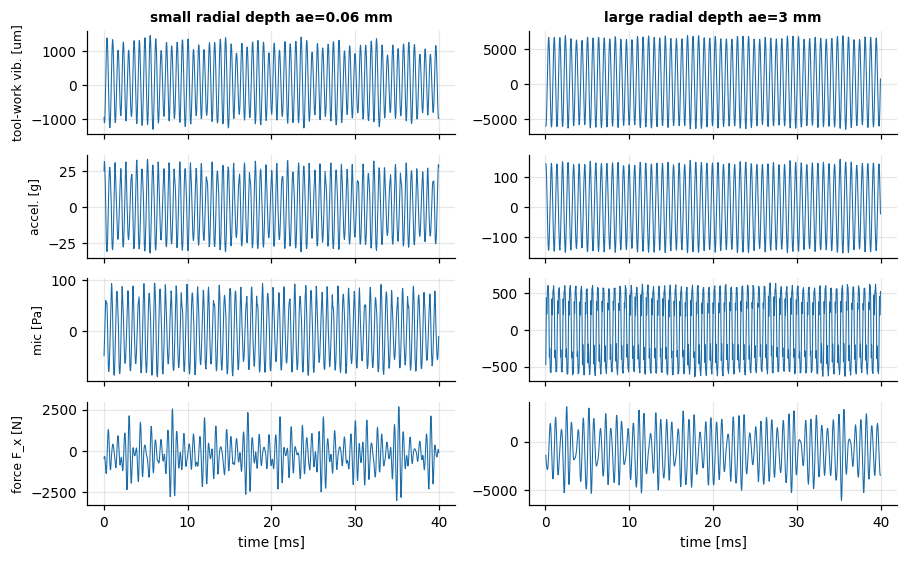
\includegraphics[width=0.95\linewidth]{figures/f_waveforms.png}
\caption{Simulated four-sensor signals at nominal parameters for the two extreme radial depths of the real data (10\,000~rpm, 2-flute 6.35~mm tool, $a_p{=}38.1$~mm). The amplitudes (millimetre-scale displacement, tens to hundreds of $g$) are not physical for stable cutting; see Section~\ref{sec:regime}.}\label{fig:waveforms}
\end{figure}

\subsection{Provenance of every parameter and the nominal operating regime}\label{sec:regime}
Following a fixed policy, a parameter is \emph{fixed} if a verified source gives its value for this exact tool and context, taken from a \emph{range} if a source gives one, and \emph{learned} from data otherwise; values with no source or data are \emph{assumed} (Figure~\ref{fig:prov}, Appendix~\ref{app:registry}). Cutting-force coefficients, tool-tip dynamics and imbalance for the simulated tool had no usable source and our attempts to learn them failed (Section~\ref{sec:neg}), so they are nominal values (Appendix~\ref{app:simparams}).
\begin{figure}[t]\centering
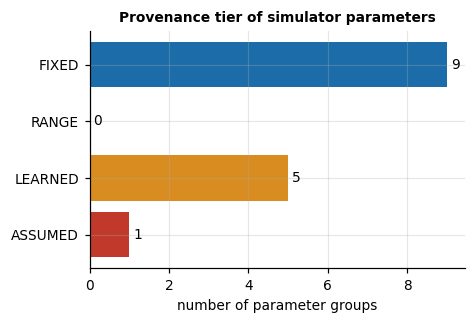
\includegraphics[width=0.5\linewidth]{figures/f_provenance.png}
\caption{Provenance tiers of the simulator parameter groups.}\label{fig:prov}
\end{figure}
\paragraph{Consequence found late: the nominal simulator is above its own stability limit.} At nominal parameters (modal stiffness $3\times10^{6}$~N/m, $f_n{=}1500$~Hz, $\zeta{=}0.03$, $K_t{=}7\times10^{8}$~N/m$^2$) the zero-order limit depth at 9000~rpm is 30.6~mm for $a_e{=}0.0635$~mm and 18.0~mm for $a_e{=}0.3175$~mm, below the real axial depth of 38.1~mm; the time-domain rms displacement is 0.44 and 0.82~mm and the tool leaves the cut ($h_{\min}=0$). Increasing the modal stiffness 3, 10 and 30 times moves the limit above the depth and the rms displacement to 36--159, 5--8 and $\le$1~$\mu$m (Table~\ref{tab:regime}). Real healthy cuts are presumably stable, so the nominal simulation is not an operating point of the real machine. Because the simulator only supplies fault \emph{differences}, which are rescaled by gains $g_\text{acc}=7.7\times10^{-6}$ and $g_\text{mic}=0.0116$ chosen to match real effect sizes, the gains absorb this amplitude mismatch (Section~\ref{sec:fault}); the structure of the simulated differences, however, is that of perturbations around a saturated limit cycle. Section~\ref{sec:k10} repeats the main benchmark with a stable-regime parameter set.
\begin{table}[t]\centering\small
\caption{Operating regime of the simulator at 9000~rpm, $a_p=38.1$~mm, as a function of the modal stiffness scale (nominal $=1$). Source: \texttt{regime\_check.py}.}\label{tab:regime}
\begin{tabular}{ccccc}
\toprule
Stiffness scale & $a_e$ [mm] & ZOA $a_{\lim}$ [mm] $\uparrow$ & $x$ rms [$\mu$m] $\downarrow$ & $F_x$ rms [N] \\
\midrule
1 & 0.0635 & \cellcolor{red!18}30.6 & 439.7 & 425 \\
1 & 0.3175 & \cellcolor{red!18}18.0 & 821.8 & 659 \\
\midrule
3 & 0.0635 & 91.7 & 36.4 & 105 \\
3 & 0.3175 & 53.7 & 159.1 & 387 \\
\midrule
10 & 0.0635 & 195.1 & 4.7 & 56 \\
10 & 0.3175 & 179.8 & 8.0 & 76 \\
\midrule
30 & 0.0635 & $>200$ & 0.7 & 52 \\
30 & 0.3175 & $>200$ & 0.9 & 58 \\
\bottomrule
\end{tabular}

\end{table}

%% =============================================================================================
\section{Healthy Baseline, Fault Injection and Features}
\subsection{Healthy baseline from real spectra}\label{sec:base}
\paragraph{Motivation.} Fitting the simulator's absolute signal levels directly to real windows did not converge (Section~\ref{sec:neg}), and the preceding section explains why the nominal simulator cannot supply a realistic healthy signal; the data constrain the \emph{healthy signal} far better than the physics constants.
\paragraph{Design.} For each 0.3~s window we compute the power spectral density of two accelerometer channels and the microphone and summarise it by a piecewise-linear envelope over log-frequency (18 knots, band-averaged linear power so that energy is preserved) plus the rms of the first eight harmonics of the spindle frequency. Envelope parameters are regressed on the cutting conditions (kernel ridge on $\log n$, $\log a_e$, $\log f$, direction); out-of-fold residuals are split by one-way variance analysis into between-cut and within-cut parts on twelve principal directions. Windows are synthesised by shaping complex Gaussian spectra with the envelope and adding harmonics with random phases (real spectra in Figure~\ref{fig:psd}).
\paragraph{Advantage.} The healthy part of a simulated window is real-data-driven, so any remaining difference to real data (Section~\ref{sec:healthy}) is attributable to the baseline model, not to the physics.
\begin{figure}[t]\centering
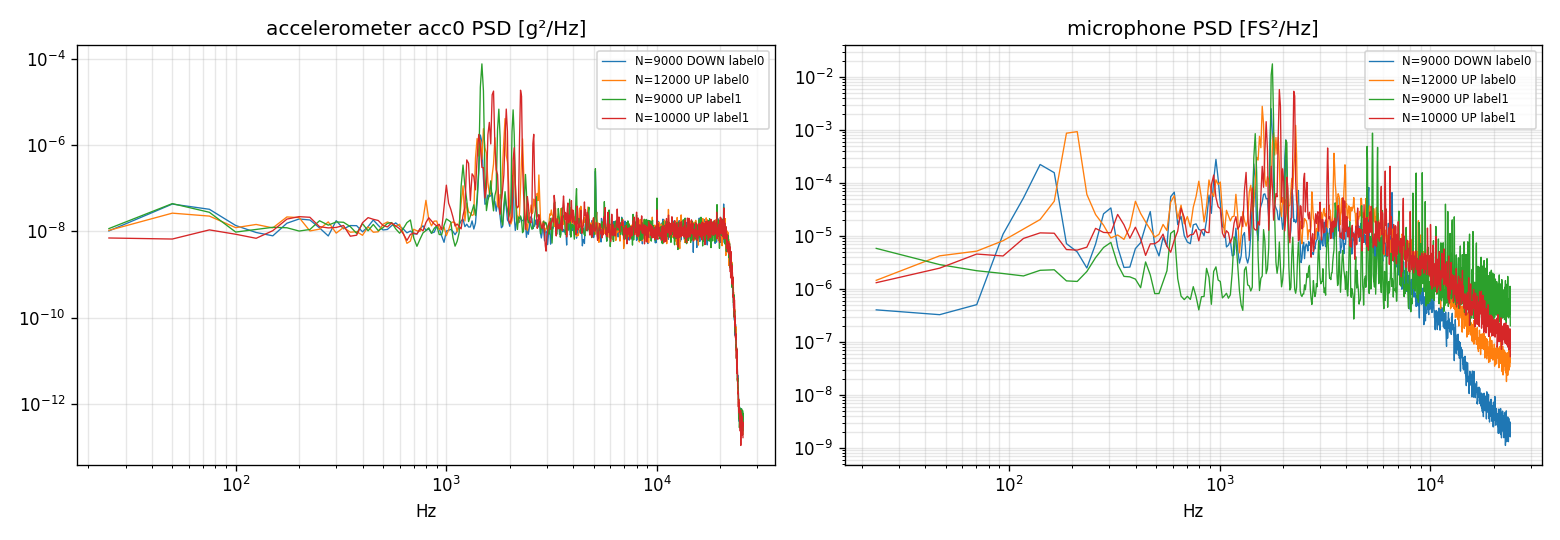
\includegraphics[width=0.95\linewidth]{figures/real_psd_examples.png}
\caption{Power spectral density of four real windows (accelerometer left, microphone right): normal and abnormal cuts at different spindle speeds.}\label{fig:psd}
\end{figure}

\subsection{Fault injection with effect-size gain}\label{sec:fault}
\paragraph{Motivation.} A simulator's absolute fault amplitude is unknown, but the \emph{direction} of a fault's effect on the signal is physically constrained.
\paragraph{Design.} For each window and fault we run the simulator twice with the same condition and noise seed and add $g\,(s_\text{fault}-s_\text{healthy})$ to the baseline, with separate $g_\text{acc},g_\text{mic}$. Faults and ranges (assumed): stiffness $\times[0.4,0.9]$ (natural frequency $\propto\sqrt{k}$); damping $\times[0.3,0.8]$; tool wear $K_t\times[1.1,1.6]$ with $K_{te},K_{re}\times(1+3(s-1))$; radial depth $\times[1.5,4]$; spindle speed $\pm[3,15]\%$. Matching feature distributions did not identify the gains (flat objective), so we set them by effect size: the mean shift of $\log_{10}$ acceleration rms and microphone level equals the real abnormal--normal difference ($+0.375$ and $+4.86$~dB), giving $g_\text{acc}=7.7\times10^{-6}$ and $g_\text{mic}=0.0116$.
\paragraph{Limit.} Real abnormal windows are mainly up-milling cuts, so the scale is an assumption about fault strength, not an estimate (Section~\ref{sec:sweep}).

\subsection{Features}
Each window is described by 30 features: log$_{10}$ acceleration rms, microphone level (dB), two spectral non-synchronous indices, ten log band powers each for the accelerometer and the microphone, the kurtosis of both, and the logarithms of spindle speed, radial depth and feed together with the milling direction.

%% =============================================================================================
\section{Root Cause Analysis Methods}\label{sec:rca}
\subsection{Problem and protocol}
Following the root-cause-ranking protocol of \citet{lee2026brcd}, a healthy dataset $D_\text{obs}$ and $m$ anomalous samples $D_\text{int}$ are given, the failure is treated as an intervention on one root-cause node, and each algorithm returns a ranking of the nodes; we report top-$k$ accuracy of the true root-cause node (chance $k/14$). Cuts are split by identity into 43 training and 30 test cuts (stratified by $a_e$); each point averages 100 random draws of $m$ faulty windows per fault, and all nodes are standardised with $D_\text{obs}$ so that no algorithm benefits from scale differences.

\subsection{Nodes and graph}
The graph has 14 nodes (Figure~\ref{fig:graph}, Table~\ref{tab:nodes}): five root-cause nodes and nine sensor nodes (log acceleration, microphone level, two non-synchronous indices, three accelerometer and two microphone bands). The directed edges (19) encode physical prior knowledge: each root cause points to the sensor quantities it can affect. Four root-cause nodes are soft sensors, i.e.\ gradient-boosted regressors of the log fault factor trained on training cuts only (out-of-fold predictions for $D_\text{obs}$); the spindle-speed node is the controller-measured deviation.
\begin{figure}[t]\centering
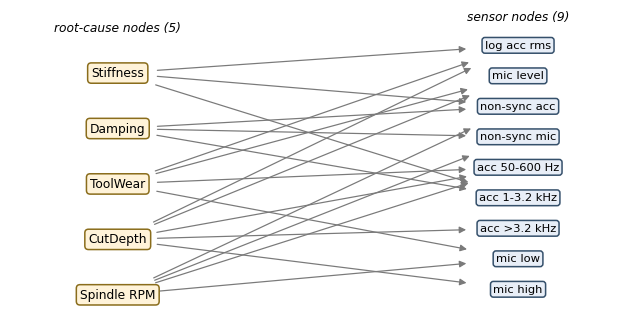
\includegraphics[width=0.72\linewidth]{figures/f_graph.png}
\caption{Causal graph used by the RCA algorithms: five root-cause nodes (left) and nine sensor nodes (right); 19 edges from physical prior knowledge.}\label{fig:graph}
\end{figure}
\begin{table}[t]\centering\small
\caption{Root-cause nodes.}\label{tab:nodes}
\begin{tabular}{llll}
\toprule
Root-cause node & Source & Quantity & Construction \\
\midrule
Stiffness\_est & soft sensor & log stiffness factor & gradient boosting on 30 spectral features \\
Damping\_est & soft sensor & log damping factor & same \\
ToolWear\_est & soft sensor & log wear factor ($K_t$) & same \\
CutDepth\_est & soft sensor & log radial-depth factor & same \\
SpindleRPM\_est & controller & log$(N/N_\text{plan})$ & true value + 0.5\% read noise \\
\bottomrule
\end{tabular}

\end{table}

\subsection{The algorithms as implemented}
Table~\ref{tab:algs} compares each algorithm with its description in \citet{lee2026brcd} (Appendix~C of that paper) and states what our code (\texttt{run\_full\_paper\_benchmark.py}) does. \textbf{The implementations are simplified, graph-aware re-implementations, not the authors' code}: all of them score a node by the standardised shift of its mean or of its residual given its parents, under a linear-Gaussian model, and BRCD, RCG, RCD and Smooth Traversal use the known graph. BARO's scoring step and SimpleRCA match their published descriptions. BRCD, RCG, RCD and Smooth Traversal contain constants with no source (0.12, 0.40, 0.70, 0.05). Consequently, our accuracies describe these re-implementations on this benchmark and must not be read as the performance of the original algorithms; the finding that the graph is irrelevant is partly a property of the re-implementations (Section~\ref{sec:circ}).
\begin{table}[t]\centering\footnotesize
\caption{The six RCA algorithms: original method (as summarised by \citealt{lee2026brcd}) versus our implementation.}\label{tab:algs}
\begin{tabular}{p{1.8cm}p{4.4cm}p{5.2cm}p{2.1cm}}\toprule
Algorithm & Original method & Our implementation & Fidelity\\\midrule
BRCD \citep{lee2026brcd} & Bayesian posterior over root causes from a CPDAG learned pre-failure, uniform DAG sampling per interventional Markov equivalence class; consistency guarantees & Linear-Gaussian local model per node on a given DAG; score = standardised mean shift of the node (root) or of its residual given parents (child), $\times(1+0.12\,|\text{descendants}|)$ & heuristic; no DAG sampling\\
RCD \citep{ikram2022rcd} & random partitions; conditional-independence tests of the failure indicator $F$ against each metric; rank by $p$-values & partial correlation test of $F$ and the node given its parents in the known DAG; score $-\log_{10}p$ & simplified; uses the true DAG\\
RCG \citep{ikram2025rcg} & marginal tests with $F$, then conditional mutual information given possible parents in a CPDAG & squared standardised shift of the residual given parents (Gaussian proxy for CMI) & simplified proxy\\
Smooth Traversal \citep{orchard2025} & outlier score of the anomalous sample; traverse from the trigger to ancestors; largest score difference between a node and its parents & mean $|z|$ score; $z_i-0.70\max_{p\in\text{pa}(i)}z_p$, plus $0.05\,z_i$ & heuristic constants\\
BARO \citep{pham2024baro} & Bayesian online change-point detection of anomaly time; rank by median/IQR-scaled deviation & median/IQR-scaled deviation with the anomaly time known & scoring step matches\\
SimpleRCA \citep{fang2025simplerca} & 95th percentile of normal data versus maximum of anomalous data & same & matches\\\bottomrule
\end{tabular}
\end{table}

\begin{algorithm}[t]
\caption{Benchmark loop for one fault, condition and number of samples $m$.}\label{alg:bench}
\begin{algorithmic}[1]
\REQUIRE healthy windows $\mathcal H$, faulty windows $\mathcal F_c$ of cause $c$, soft sensors $\{g_j\}$, graph $G$, algorithm $\mathcal A$
\STATE $D_\text{obs}\leftarrow$ nodes of $\mathcal H$ (soft sensors out-of-fold), standardise with its mean and s.d.
\FOR{trial $=1,\dots,100$}
\STATE draw $m$ windows from $\mathcal F_c$ with replacement if needed; compute nodes with $g_j$; standardise $\to D_\text{int}$
\STATE ranking $\leftarrow\mathcal A(D_\text{obs},D_\text{int},G)$
\STATE record whether $\text{node}(c)$ is at rank 1, within 3, within 5
\ENDFOR
\RETURN mean top-1/3/5 over trials and over the five causes
\end{algorithmic}
\end{algorithm}

\subsection{Generator shift}
Because the soft sensors are trained on labels from the same generator, a \emph{shifted} test multiplies natural frequency, damping, stiffness, force and edge coefficients by random factors in $[0.75,1.33]$, $[0.5,2]$, $[0.6,1.7]$, $[0.6,1.6]$ and $[0.4,2.5]$ per cut, with soft sensors left at their nominal training.

%% =============================================================================================
\section{Experiments}
\subsection{Is the benchmark circular? Generator shift and ablations}\label{sec:circ}
\paragraph{Question and protocol.} Does the accuracy of the causal RCA algorithms reflect diagnosis, or the match between nodes and generator? We compare shared-generator and shifted settings (Table~\ref{tab:causal}, Figures~\ref{fig:mcurve}, \ref{fig:heat}) and ablate graph and node construction (Table~\ref{tab:ablation}, Figure~\ref{fig:ablation}; three seeds, each changing the cut split and data; 60 draws per fault).
\begin{table}[t]\centering\small
\caption{Causal RCA: top-1 accuracy $\uparrow$ (mean over 5 root causes; 100 draws per fault) versus the number of anomalous samples $m$; best per column in bold.}\label{tab:causal}
\begin{tabular}{l cccc cccc}
\toprule
& \multicolumn{4}{c}{Same generator} & \multicolumn{4}{c}{Shifted generator parameters} \\
\cmidrule(lr){2-5}\cmidrule(lr){6-9}
Algorithm & $m{=}5$ & $10$ & $20$ & $50$ & $m{=}5$ & $10$ & $20$ & $50$ \\
\midrule
BRCD & 0.87 & 0.90 & 0.89 & 0.85 & 0.59 & 0.58 & 0.62 & 0.64 \\
RCD & 0.79 & 0.80 & 0.71 & 0.59 & 0.45 & 0.39 & 0.30 & 0.21 \\
RCG & 0.87 & 0.90 & 0.89 & 0.85 & 0.58 & 0.59 & 0.63 & 0.64 \\
Smooth Traversal & \cellcolor{gray!20}\textbf{0.95} & \cellcolor{gray!20}\textbf{0.98} & \cellcolor{gray!20}\textbf{1.00} & \cellcolor{gray!20}\textbf{1.00} & \cellcolor{gray!20}\textbf{0.68} & \cellcolor{gray!20}\textbf{0.71} & \cellcolor{gray!20}\textbf{0.77} & \cellcolor{gray!20}\textbf{0.81} \\
BARO & 0.88 & 0.94 & 0.98 & 1.00 & 0.42 & 0.35 & 0.30 & 0.26 \\
SimpleRCA & 0.53 & 0.52 & 0.52 & 0.48 & 0.42 & 0.44 & 0.44 & 0.40 \\
\midrule
Chance (1/14) & 0.07 & 0.07 & 0.07 & 0.07 & 0.07 & 0.07 & 0.07 & 0.07 \\
\bottomrule
\end{tabular}

\end{table}
\begin{figure}[t]\centering
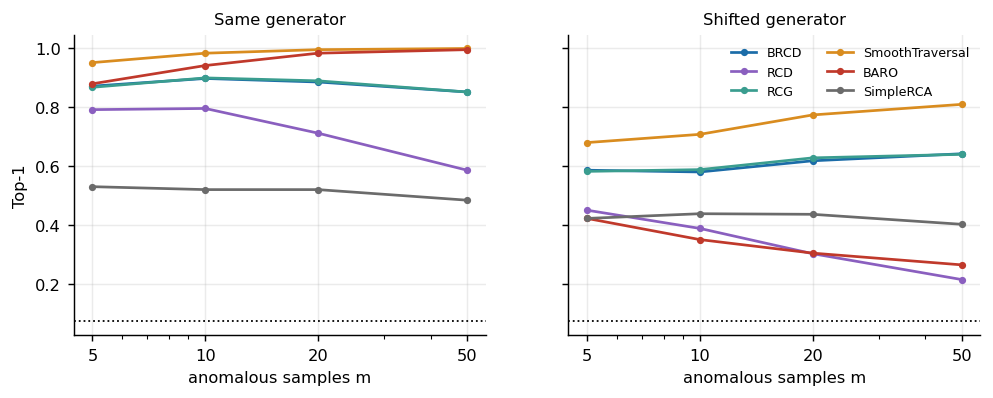
\includegraphics[width=0.95\linewidth]{figures/f_m_curve.png}
\caption{Top-1 accuracy versus the number of anomalous samples in the shared-generator and shifted settings (dotted: chance). In the shifted setting BARO and RCD deteriorate with more samples while Smooth Traversal improves.}\label{fig:mcurve}
\end{figure}
\paragraph{Generator shift.} With a shared generator, Smooth Traversal and BARO approach 1.0 as $m$ grows, BRCD and RCG reach 0.85--0.90, RCD declines with $m$, and SimpleRCA stays near 0.5. Under shifted parameters all methods drop and the ordering changes: BARO falls from 0.94 to 0.35 at $m{=}10$, BRCD and RCG improve slowly with $m$, and Smooth Traversal remains best at 0.71 (top-3: 0.98 Smooth Traversal, 0.93 BARO, 0.89 BRCD). Figure~\ref{fig:heat} shows that the accuracy is unevenly spread over the causes.
\begin{figure}[t]\centering
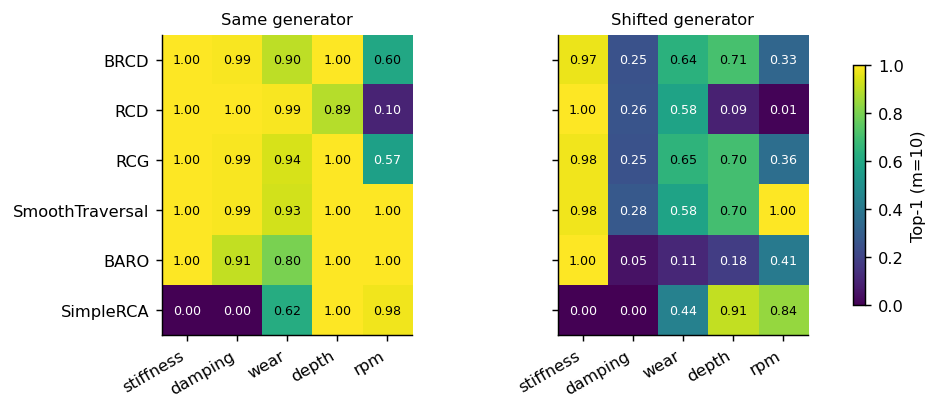
\includegraphics[width=0.95\linewidth]{figures/f_cause_heatmap.png}
\caption{Top-1 accuracy per root cause and algorithm at $m{=}10$.}\label{fig:heat}
\end{figure}
\paragraph{Graph and node ablation.} Replacing the physical graph by random edges of equal out-degree or by an empty graph changes no algorithm beyond the seed spread (BRCD $0.92\pm0.01$, $0.92\pm0.02$, $0.92\pm0.00$ shared; $0.60\pm0.05$, $0.60\pm0.05$, $0.58\pm0.06$ shifted). Every root-cause node is a graph root, so in our re-implementations the conditional models cannot add information about it and the methods act as marginal shift detectors on the node estimates, consistent with the observation of \citet{lee2026brcd} on BARO and SimpleRCA. Replacing the supervised soft sensors by label-free spectral summaries reduces accuracy to $0.07$--$0.29$ (shared) and $0.07$--$0.37$ (shifted); the simplest method reaches exactly $0.20$, consistent with only the controller-measured speed node remaining informative (not tested directly). Under shift, a threefold larger fault gain lowers accuracy (BRCD $0.60\to0.27$, Smooth Traversal $0.71\to0.28$) because soft sensors trained on nominal parameters mis-estimate larger, distorted effects.
\begin{table}[t]\centering\footnotesize
\caption{Ablation at $m{=}10$: top-1 accuracy $\uparrow$ (mean $\pm$ s.d.\ over 3 seeds); chance $=0.07$.}\label{tab:ablation}
\begin{tabular}{p{5.6cm}cccccc}
\toprule
Variant & BRCD & RCD & RCG & Smooth & BARO & Simple \\
\midrule
\multicolumn{7}{l}{\textit{Same generator}} \\
\quad Supervised nodes, physics graph (main) & 0.92\,$\pm$\,0.01 & 0.81\,$\pm$\,0.03 & 0.92\,$\pm$\,0.01 & 0.99\,$\pm$\,0.00 & 0.91\,$\pm$\,0.07 & 0.54\,$\pm$\,0.00 \\
\quad Supervised nodes, shuffled graph & 0.92\,$\pm$\,0.02 & 0.81\,$\pm$\,0.03 & 0.92\,$\pm$\,0.01 & 0.99\,$\pm$\,0.00 & 0.91\,$\pm$\,0.07 & 0.54\,$\pm$\,0.00 \\
\quad Supervised nodes, no edges & 0.92\,$\pm$\,0.00 & 0.81\,$\pm$\,0.02 & 0.92\,$\pm$\,0.00 & 0.99\,$\pm$\,0.00 & 0.91\,$\pm$\,0.07 & 0.54\,$\pm$\,0.00 \\
\quad Label-free nodes, physics graph & 0.09\,$\pm$\,0.01 & 0.10\,$\pm$\,0.04 & 0.07\,$\pm$\,0.01 & 0.29\,$\pm$\,0.08 & 0.29\,$\pm$\,0.08 & 0.20\,$\pm$\,0.00 \\
\quad Supervised, physics graph, gain $\times0.3$ & 0.85\,$\pm$\,0.02 & 0.78\,$\pm$\,0.04 & 0.85\,$\pm$\,0.02 & 0.88\,$\pm$\,0.05 & 0.65\,$\pm$\,0.18 & 0.51\,$\pm$\,0.01 \\
\quad Supervised, physics graph, gain $\times3$ & 0.85\,$\pm$\,0.02 & 0.76\,$\pm$\,0.05 & 0.84\,$\pm$\,0.02 & 0.99\,$\pm$\,0.01 & 0.97\,$\pm$\,0.01 & 0.53\,$\pm$\,0.04 \\
\midrule
\multicolumn{7}{l}{\textit{Shifted generator parameters}} \\
\quad Supervised nodes, physics graph (main) & 0.60\,$\pm$\,0.05 & 0.43\,$\pm$\,0.05 & 0.60\,$\pm$\,0.07 & 0.71\,$\pm$\,0.07 & 0.39\,$\pm$\,0.05 & 0.45\,$\pm$\,0.01 \\
\quad Supervised nodes, shuffled graph & 0.60\,$\pm$\,0.05 & 0.42\,$\pm$\,0.05 & 0.59\,$\pm$\,0.06 & 0.71\,$\pm$\,0.07 & 0.40\,$\pm$\,0.05 & 0.45\,$\pm$\,0.01 \\
\quad Supervised nodes, no edges & 0.58\,$\pm$\,0.06 & 0.42\,$\pm$\,0.05 & 0.58\,$\pm$\,0.06 & 0.70\,$\pm$\,0.06 & 0.39\,$\pm$\,0.06 & 0.45\,$\pm$\,0.01 \\
\quad Label-free nodes, physics graph & 0.09\,$\pm$\,0.01 & 0.14\,$\pm$\,0.04 & 0.07\,$\pm$\,0.01 & 0.27\,$\pm$\,0.03 & 0.37\,$\pm$\,0.02 & 0.20\,$\pm$\,0.00 \\
\quad Supervised, physics graph, gain $\times0.3$ & 0.54\,$\pm$\,0.03 & 0.45\,$\pm$\,0.05 & 0.53\,$\pm$\,0.03 & 0.59\,$\pm$\,0.03 & 0.48\,$\pm$\,0.02 & 0.42\,$\pm$\,0.02 \\
\quad Supervised, physics graph, gain $\times3$ & 0.27\,$\pm$\,0.07 & 0.22\,$\pm$\,0.01 & 0.26\,$\pm$\,0.07 & 0.28\,$\pm$\,0.09 & 0.22\,$\pm$\,0.01 & 0.32\,$\pm$\,0.07 \\
\bottomrule
\end{tabular}

\end{table}
\begin{figure}[t]\centering
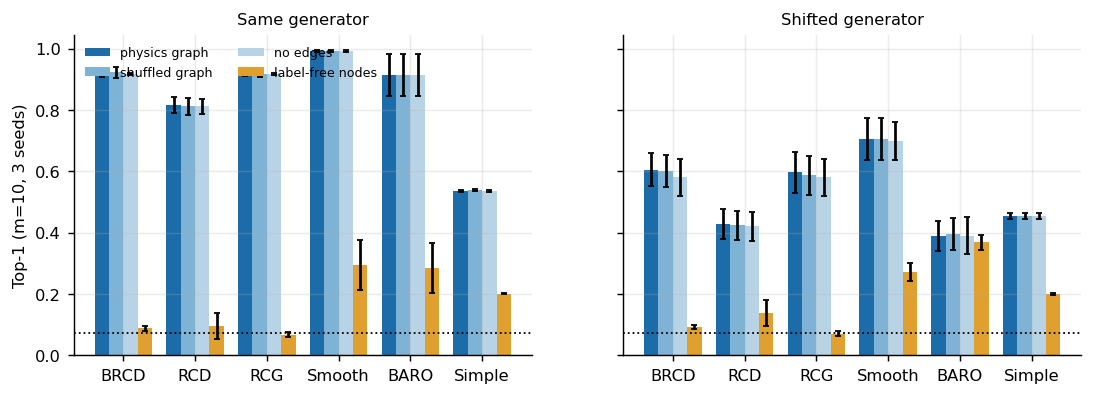
\includegraphics[width=0.95\linewidth]{figures/f_ablation.png}
\caption{Ablation at $m{=}10$ (mean $\pm$ s.d.\ over 3 seeds): the graph does not matter; node construction does.}\label{fig:ablation}
\end{figure}
\paragraph{Reading.} The benchmark measures supervised estimation of the root-cause nodes and its sensitivity to generator mismatch, not causal reasoning.

\subsection{How far is the simulated healthy baseline from real data?}\label{sec:healthy}
We train the baseline on a subset of cuts and test on held-out cuts with a random-forest classifier two-sample test (balanced accuracy, folds by cut; 0.5 means indistinguishable). Table~\ref{tab:c2st} and Figure~\ref{fig:c2st} show that all variants remain far from 0.5 ($0.82\pm0.04$ for the final model) and that the kernel and hierarchical improvements are small relative to the split spread. Feature means match (log acceleration $-1.37$ simulated, $-1.38$ real) but dispersion and joint dependence on conditions do not. We could not measure a floor because no cutting condition is repeated. An earlier version used plain accuracy with five synthetic windows per real one (chance 0.83); those numbers are discarded.
\begin{table}[t]\centering\small
\caption{Classifier two-sample test, real versus simulated healthy windows on held-out cuts (3 random stratified splits, mean $\pm$ s.d.; 22 test cuts).}\label{tab:c2st}
\begin{tabular}{llc}
\toprule
Mean model & Variation model & C2ST balanced accuracy $\downarrow$ \\
\midrule
Linear & mean only & 0.946 $\pm$ 0.025 \\
Linear & + between/within-cut variation & 0.853 $\pm$ 0.022 \\
Kernel ridge & mean only & 0.864 $\pm$ 0.022 \\
Kernel ridge & + between/within-cut variation (final) & \cellcolor{gray!20}\textbf{0.820 $\pm$ 0.036} \\
\bottomrule
\end{tabular}

\end{table}
\begin{figure}[t]\centering
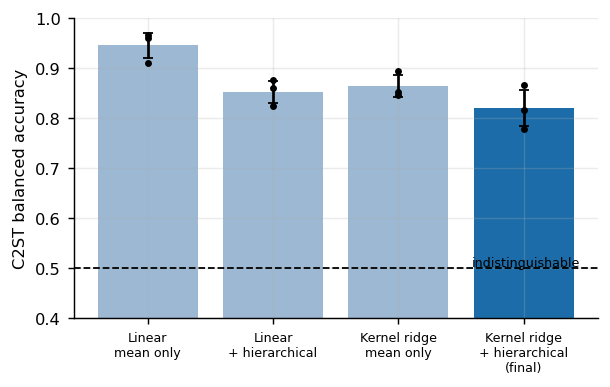
\includegraphics[width=0.5\linewidth]{figures/f_c2st.png}
\caption{C2ST balanced accuracy of the four baseline variants (dots: individual splits; dashed: indistinguishable).}\label{fig:c2st}
\end{figure}

\subsection{Negative result: direct calibration of the delay model}\label{sec:neg}
Fitting 15 physical and sensor parameters to real windows with CMA-ES (MMD, later group means over conditions) plateaued at a loss near 3 (squared errors in real standard deviations) and did not converge in 35--40 generations; we stopped by a pre-set rule. Earlier low-MMD fits had wrong dependence on conditions: real microphone level correlates with spindle speed at $+0.85$, the simulation gave $0.00$; simulated acceleration depended on radial depth ($0.69$), the real one did not ($0.06$). A window-length mismatch (4~s real versus 0.18~s simulated) had inflated simulated variance threefold. The data do not constrain the delay model's absolute levels, hence the use of fault \emph{differences}.

\subsection{Does any simulated fault reproduce a real defective tool?}\label{sec:real}
\paragraph{Protocol.} We compare the intentionally defective tool D$^*$ (12 cuts, 36 windows) with the healthy tool of the same type (64 cuts, 192 windows). Conditions differ, so we fit ridge models of each sensor node on the conditions with healthy cuts only (out-of-sample over cuts), express defective windows as residuals in healthy standard deviations, and bootstrap cuts for 95\% intervals (Table~\ref{tab:realshift}, Figure~\ref{fig:sig}).
\begin{table}[t]\centering\footnotesize
\caption{Shift of each sensor node in healthy standard deviations: real defective tool D$^*$ (95\% bootstrap interval over cuts) versus five simulated faults. Red (blue) cells: shift $\ge2$ ($\le-2$) s.d.}\label{tab:realshift}
\begin{tabular}{lcccccc}
\toprule
& Real tool D$^*$ & \multicolumn{5}{c}{Simulated fault} \\
\cmidrule(lr){3-7}
Sensor node [s.d.] & [95\% CI] & Stiff. & Damp. & Wear & Depth & RPM \\
\midrule
log acc.\ rms & +1.9 [+1.4, +2.5] & \cellcolor{red!18}+2.9 & \cellcolor{red!18}+2.9 & +1.9 & \cellcolor{red!18}+2.9 & \cellcolor{red!18}+3.0 \\
mic.\ level & \cellcolor{red!18}+3.6 [+3.2, +4.1] & \cellcolor{red!18}+2.3 & \cellcolor{red!18}+2.4 & +1.4 & \cellcolor{red!18}+2.3 & \cellcolor{red!18}+2.4 \\
non-sync.\ index (acc) & \cellcolor{blue!15}-3.7 [-4.3, -3.1] & -0.0 & -0.3 & -0.3 & -0.2 & +0.3 \\
non-sync.\ index (mic) & -1.2 [-1.5, -0.9] & +0.1 & -0.2 & -0.2 & -0.2 & +0.5 \\
acc.\ 50--600\,Hz & \cellcolor{red!18}+3.9 [+3.5, +4.2] & -0.0 & +0.0 & -0.0 & -0.0 & +0.0 \\
acc.\ 1--3.2\,kHz & \cellcolor{red!18}+6.3 [+5.6, +7.1] & +1.8 & +1.2 & +1.0 & +1.3 & +1.5 \\
acc.\ $>$3.2\,kHz & +1.9 [+1.4, +2.3] & +1.5 & +1.3 & +1.5 & \cellcolor{red!18}+2.1 & \cellcolor{red!18}+2.1 \\
mic.\ 50--600\,Hz & \cellcolor{red!18}+4.0 [+3.3, +4.7] & -0.0 & +0.0 & +0.0 & -0.0 & +0.1 \\
mic.\ $>$3.2\,kHz & +1.8 [+1.2, +2.3] & +0.2 & +0.2 & +0.1 & +0.3 & +0.3 \\
\midrule
Cosine with real shift & -- & 0.62 & 0.60 & 0.62 & 0.59 & 0.55 \\
\bottomrule
\end{tabular}

\end{table}
\begin{figure}[t]\centering
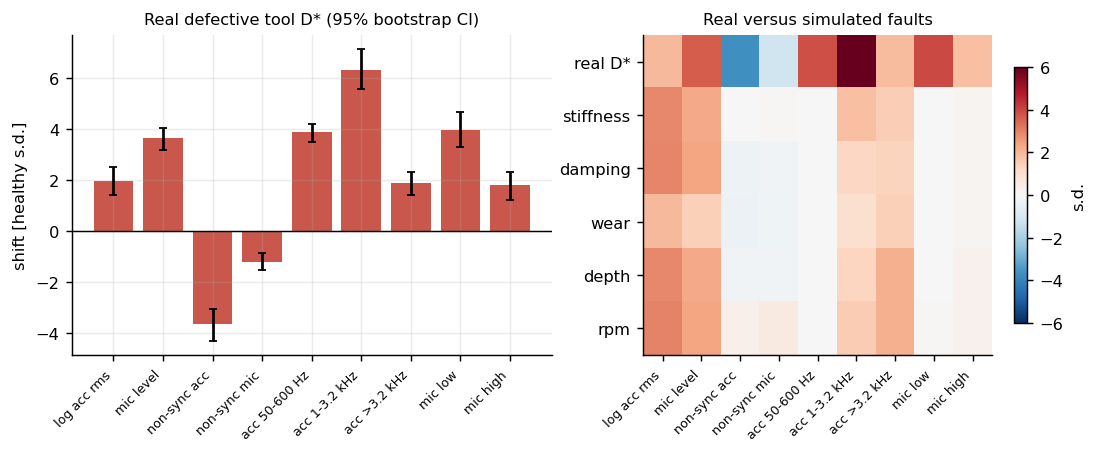
\includegraphics[width=0.97\linewidth]{figures/f_signature.png}
\caption{Left: real defective-tool shift with 95\% bootstrap intervals. Right: real versus simulated fault shifts on the same scale. Simulated faults raise broadband levels but do not move the low-frequency bands or the non-synchronous indices.}\label{fig:sig}
\end{figure}
\paragraph{Result.} The real tool raises all levels, most at low frequency ($+3.9$ and $+4.0$ for the 50--600~Hz accelerometer and microphone bands) and in the 1--3.2~kHz accelerometer band ($+6.3$), and lowers both non-synchronous indices ($-3.7$, $-1.2$), i.e.\ the spectrum becomes more tonal. No simulated fault shifts low frequencies (all within $\pm0.1$) or the non-synchronous indices beyond $-0.3$ to $+0.5$. The cosine similarity to the five simulated shifts is $0.55$--$0.62$ and driven by the common ``louder'' direction.
\paragraph{Tested hypothesis: chipped flute.} We added effective runout of 10--80~$\mu$m (a once-per-revolution term) and tried fault gains of $1\times$, $10\times$, $100\times$ (Figure~\ref{fig:chip}). The cosine similarity stays at $0.48$--$0.54$, again dominated by overall level; non-synchronous indices move in the wrong direction ($+0.1$ to $+0.9$ versus $-3.7$ and $-1.2$), the low bands barely change (microphone low band $\le+0.9$ versus $+4.0$), and the high accelerometer band grows far too much with added gain ($+1$ to $+38$ versus $+1.9$). A once-per-revolution runout therefore does not reproduce the signature either. Per-tooth force asymmetry and nonlinear edge or friction effects remain untested.
\begin{figure}[t]\centering
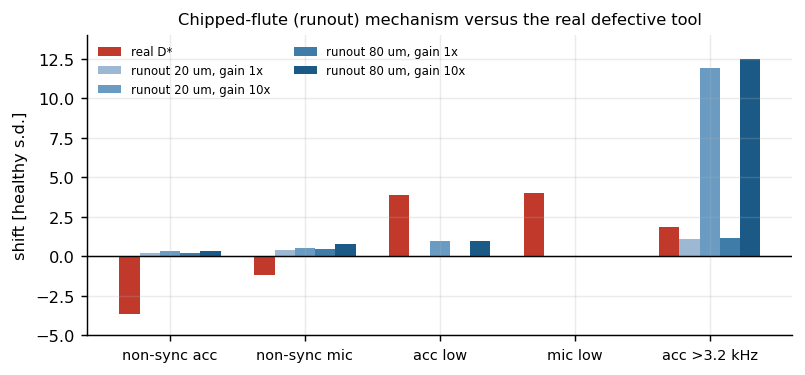
\includegraphics[width=0.78\linewidth]{figures/f_chipped.png}
\caption{Chipped-flute test: shifts of five discriminating nodes for the real defective tool (red) and for simulated effective runout of 20 and 80~$\mu$m at fault gains $1\times$ and $10\times$.}\label{fig:chip}
\end{figure}
\paragraph{Scope.} The tools differ (12.7~mm four-flute steel versus simulated 6.35~mm two-flute aluminium), so only direction and sign in standardised units are compared.

\subsection{Sensitivity to the assumed fault strength}\label{sec:sweep}
Scaling the fault gains by $0.3$ and $3$ changes the best simulated classifier's accuracy from $0.698$ to $0.943$ (Table~\ref{tab:sweep}, Figure~\ref{fig:gain}); six-class accuracy within the simulator (Table~\ref{tab:cls}, 16 held-out cuts) is therefore only interpretable together with this curve. Applied to real windows, 91--97\% of normal windows are classified normal by tree and neighbour models but only 51\% and 57\% by logistic regression and Naive Bayes, and 61, 64 and 72 of 75 real abnormal windows are assigned to tool wear by QDA, random forest and gradient boosting; with no ground truth for abnormal windows we read this as mapping any broadband increase to wear.
\begin{table}[t]\centering\small
\caption{Top-1 accuracy $\uparrow$ of classifiers on simulated data versus fault gain relative to the calibrated value.}\label{tab:sweep}
\begin{tabular}{lccc}
\toprule
Classifier & gain $\times0.3$ $\uparrow$ & $\times1$ (calibrated) $\uparrow$ & $\times3$ $\uparrow$ \\
\midrule
Gradient boosting & \cellcolor{gray!20}\textbf{0.698} & \cellcolor{gray!20}\textbf{0.882} & \cellcolor{gray!20}\textbf{0.943} \\
Random forest & 0.674 & 0.855 & 0.922 \\
QDA (Bayes) & 0.545 & 0.769 & 0.847 \\
Logistic regression & 0.535 & 0.729 & 0.834 \\
\bottomrule
\end{tabular}

\end{table}
\begin{table}[t]\centering\small
\caption{Six-class classification on simulated data, 16 held-out cuts (chance $0.167$).}\label{tab:cls}
\begin{tabular}{lcccc}
\toprule
Classifier & Top-1 $\uparrow$ & Top-3 $\uparrow$ & Macro-F1 $\uparrow$ & AUROC$_{\text{fault vs.\ normal}}$ $\uparrow$ \\
\midrule
Gradient boosting & \cellcolor{gray!20}\textbf{0.886} & \cellcolor{gray!20}\textbf{0.990} & \cellcolor{gray!20}\textbf{0.885} & \cellcolor{gray!20}\textbf{1.000} \\
Random forest & 0.870 & \cellcolor{gray!20}\textbf{0.990} & 0.868 & 0.998 \\
MLP & 0.807 & 0.987 & 0.804 & 0.994 \\
QDA (Bayes) & 0.787 & 0.978 & 0.779 & 0.992 \\
Logistic regression & 0.726 & 0.966 & 0.722 & 0.990 \\
kNN & 0.722 & 0.922 & 0.717 & 0.983 \\
Gaussian Naive Bayes & 0.579 & 0.912 & 0.554 & 0.961 \\
\bottomrule
\end{tabular}

\end{table}
\begin{figure}[t]\centering
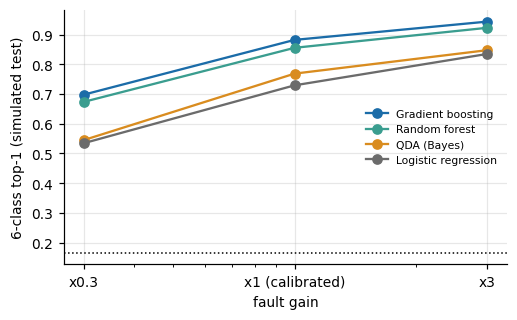
\includegraphics[width=0.55\linewidth]{figures/f_gain_sweep.png}
\caption{Simulated six-class accuracy as a function of the assumed fault gain.}\label{fig:gain}
\end{figure}

\subsection{When does simulation help on real data? Cross-machine wear}\label{sec:wear}
\paragraph{Setup.} LUH has three machines and three tools per machine with measured flank wear (VB). The target is wear $\ge100~\mu$m (AUROC; chance 0.5; 406 runs, 26\% positive). Features are force-based (means, standard deviations, kurtosis, band powers of $x$, $y$ and the resultant).
\paragraph{Baselines for unseen machines.} Table~\ref{tab:luhbase} and Figure~\ref{fig:luh} compare a one-feature rule (mean resultant force, higher means worn, no labels needed), gradient boosting, logistic regression, CORAL and DANN with 10 seeds, leaving one machine out. Wear detection is easy: gradient boosting with raw features is $\ge0.976$ on all three target machines. The one-feature rule reaches $0.996$ and $0.993$ on machines 1 and 2 but $0.46$ on machine 3, so force scale differs across machines. Domain adaptation does not improve on gradient boosting, and tool-relative features make DANN unstable (machine 1: $0.79\pm0.13$). Normalising features by each machine's healthy baseline did not raise AUROC (unseen machine, gradient boosting: $0.990$ raw, $0.955$ machine-relative, $0.986$ tool-relative) and increased the wear-estimation error (MAE of VB $9.2$, $17.7$, $11.1~\mu$m). Bootstrap intervals are over runs and understate uncertainty because runs of one tool are correlated; gradient boosting and logistic regression are deterministic, so their seed spread is zero.
\begin{table}[t]\centering\small
\caption{Leave-one-machine-out wear detection (VB $\ge100~\mu$m), AUROC $\uparrow$, mean over 10 seeds on target machines M1--M3.}\label{tab:luhbase}
\begin{tabular}{lccc}
\toprule
Method (target machine $\rightarrow$) & M1 $\uparrow$ & M2 $\uparrow$ & M3 $\uparrow$ \\
\midrule
\multicolumn{4}{l}{\textit{Raw features}} \\
\quad One-feature RMS rule (no labels) & 0.996 & 0.993 & 0.462 \\
\quad Gradient boosting & 0.995 & \cellcolor{gray!20}\textbf{0.999} & \cellcolor{gray!20}\textbf{0.976} \\
\quad Logistic regression & 0.996 & 0.995 & 0.943 \\
\quad CORAL + LR$^{\dagger}$ & 0.992 & 0.995 & 0.886 \\
\quad DANN$^{\dagger}$ & \cellcolor{gray!20}\textbf{0.996} & 0.997 & 0.974 \\
\midrule
\multicolumn{4}{l}{\textit{Machine-relative features}} \\
\quad One-feature RMS rule (no labels) & 0.996 & 0.993 & 0.462 \\
\quad Gradient boosting & 0.965 & 0.989 & 0.910 \\
\quad Logistic regression & \cellcolor{gray!20}\textbf{0.998} & \cellcolor{gray!20}\textbf{0.999} & 0.964 \\
\quad CORAL + LR$^{\dagger}$ & 0.981 & 0.952 & 0.956 \\
\quad DANN$^{\dagger}$ & 0.997 & 0.879 & \cellcolor{gray!20}\textbf{0.980} \\
\midrule
\multicolumn{4}{l}{\textit{Tool-relative features}} \\
\quad One-feature RMS rule (no labels) & 0.925 & 0.894 & 0.433 \\
\quad Gradient boosting & \cellcolor{gray!20}\textbf{0.980} & 0.994 & \cellcolor{gray!20}\textbf{0.985} \\
\quad Logistic regression & 0.931 & \cellcolor{gray!20}\textbf{0.999} & 0.946 \\
\quad CORAL + LR$^{\dagger}$ & 0.822 & 0.997 & 0.926 \\
\quad DANN$^{\dagger}$ & 0.786 & 0.998 & 0.731 \\
\midrule
Simulation only, no real labels (tool-relative $x,y$) & 0.887 & 0.807 & 0.571 \\
\bottomrule
\end{tabular}
\vspace{1pt}\\{\footnotesize $^{\dagger}$ uses unlabelled target-machine features (transductive).}

\end{table}
\begin{figure}[t]\centering
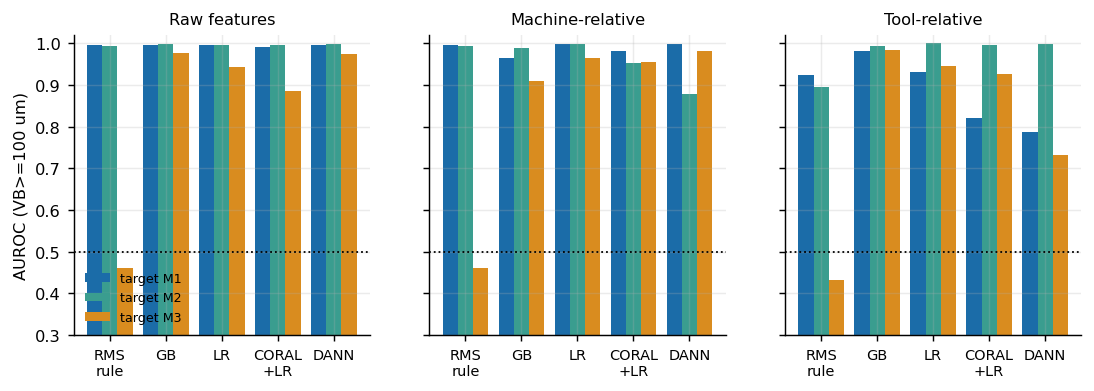
\includegraphics[width=0.97\linewidth]{figures/f_luh_baselines.png}
\caption{Leave-one-machine-out AUROC for three feature sets and five methods (dotted: chance).}\label{fig:luh}
\end{figure}
\paragraph{Simulation without real labels.} A classifier trained only on simulated wear (a four-flute DDE with randomised machine--tool parameters and randomised wear effects) and applied to the three target machines reaches AUROC $0.887$, $0.807$ and $0.571$ using sign-invariant tool-relative features. The first attempt with signed mean force was below chance ($0.55$, $0.26$, $0.10$) because of an axis sign convention; changing to absolute mean force was decided after seeing this result, though with a physical argument, so the numbers should be read as exploratory.
\paragraph{Earlier wear thresholds.} Because heavy wear may be too easy, we repeated the label-free comparison at VB $\ge60$ and $\ge40~\mu$m (thresholds fixed before running; all three are reported). The comparator is the resultant-force rule on the same tool-relative $x,y$ features (Table~\ref{tab:thr}, Figure~\ref{fig:thr}). Averaged over machines, the simulation-only model is higher than the rule at every threshold, but the gain comes from machine~3, where the rule is below chance ($0.42$, $0.40$ and $0.43$) and simulation reaches $0.57$--$0.78$; on machines 1 and 2 the rule is as good as or better than simulation in five of six cases (machine 1 at $60~\mu$m is tied). The evidence for a label-free benefit of simulation is therefore limited to one of three machines, with the sign of the one-feature rule on that machine unexplained.
\begin{table}[t]\centering\small
\caption{Label-free wear detection on unseen machines, AUROC $\uparrow$, by wear threshold. Rule: mean resultant force on tool-relative $x,y$ features.}\label{tab:thr}
\begin{tabular}{llcccc}
\toprule
VB threshold [$\mu$m] & Method & M1 $\uparrow$ & M2 $\uparrow$ & M3 $\uparrow$ & Mean $\uparrow$ \\
\midrule
\multirow{2}{*}{$\ge100$} & One-feature rule & 0.853 & 0.936 & 0.433 & 0.740 \\
 & Simulation only & 0.887 & 0.807 & 0.571 & \cellcolor{gray!20}\textbf{0.755} \\
\midrule
\multirow{2}{*}{$\ge60$} & One-feature rule & 0.927 & 0.870 & 0.415 & 0.737 \\
 & Simulation only & 0.925 & 0.809 & 0.759 & \cellcolor{gray!20}\textbf{0.831} \\
\midrule
\multirow{2}{*}{$\ge40$} & One-feature rule & 0.994 & 0.941 & 0.398 & 0.777 \\
 & Simulation only & 0.827 & 0.893 & 0.782 & \cellcolor{gray!20}\textbf{0.834} \\
\bottomrule
\end{tabular}

\end{table}
\begin{figure}[t]\centering
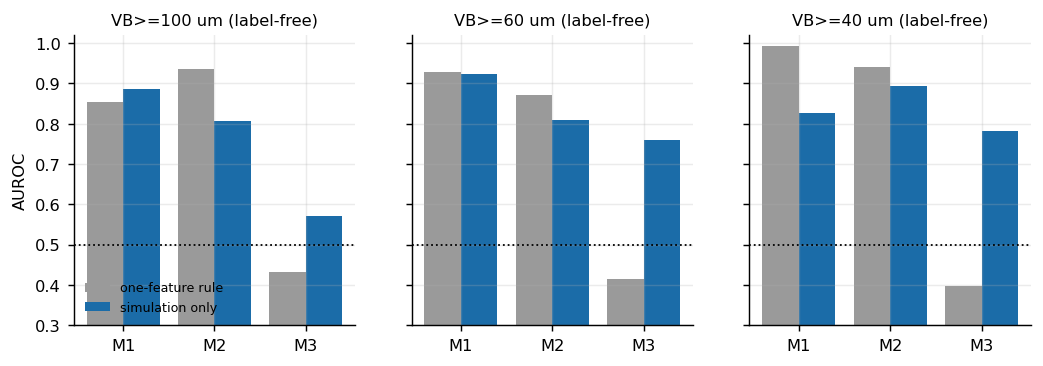
\includegraphics[width=0.97\linewidth]{figures/f_wear_threshold.png}
\caption{Label-free AUROC of the one-feature rule and the simulation-only model per machine and wear threshold.}\label{fig:thr}
\end{figure}
\paragraph{Fine-tuning.} Fine-tuning from the simulated solution with $k$ real samples was not better than training from scratch at any $k$ and any threshold (Figure~\ref{fig:ft}; at $k{=}2$, $\lambda{=}1$: $0.83$ vs.\ $0.85$ at $100~\mu$m, $0.90$ vs.\ $0.94$ at $60~\mu$m, $0.87$ vs.\ $0.97$ at $40~\mu$m). On this easy task a few real labels already suffice.
\begin{figure}[t]\centering
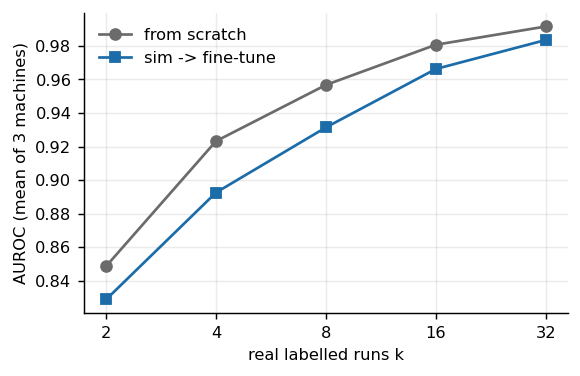
\includegraphics[width=0.5\linewidth]{figures/f_finetune.png}
\caption{AUROC versus the number $k$ of real labelled runs (VB $\ge100~\mu$m; mean of three machines).}\label{fig:ft}
\end{figure}
\paragraph{Does real-data transfer degrade when the target dynamics are far from the training machines?} Without measured transfer functions for LUH we used a proxy: the mean 21-band force spectrum of the three least-worn runs of each tool. For each of the nine target tools we trained on the tools of the other machines (all six, the three nearest, the three farthest by the proxy). With gradient boosting and raw features at VB $\ge100~\mu$m, AUROC was $0.993$, $0.984$ and $0.976$ for all, nearest and farthest training tools; the Spearman correlation between proxy distance and AUROC was $-0.16$ ($p=0.67$) at VB $\ge100~\mu$m and $-0.34$ ($p=0.36$) at $60~\mu$m (Figure~\ref{fig:dyn}). Only logistic regression on tool-relative features at $60~\mu$m showed a trend ($\rho=-0.62$, $p=0.08$; lowest AUROC $0.25$). With nine targets, a weak proxy and an unknown range of dynamics, this is absence of evidence, not evidence of absence: on these data real-data transfer is sufficient, and whether simulation is needed to reach dynamics outside the training range remains open.
\begin{figure}[t]\centering
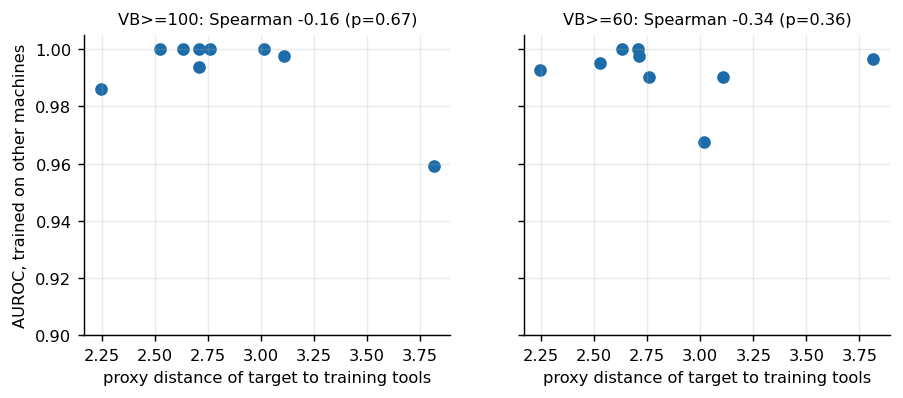
\includegraphics[width=0.78\linewidth]{figures/f_dynamics_shift.png}
\caption{Real-data transfer to an unseen machine versus the spectral proxy distance of the target tool to the training tools (nine targets).}\label{fig:dyn}
\end{figure}

\subsection{FRF import}\label{sec:frf}
For a new machine the tool-tip transfer function can be read from hammer-test data (receptance, or accelerance divided by $(j\omega)^2$) and fitted by adding modes at residual peaks with linear residue estimation. On synthetic transfer functions with added noise the shape error is 0.8\% (no noise), 1.7\% (noise 1\% of the peak) and 16\% (3\%, one mode lost); the importer has not been tested on measured FRFs (Figure~\ref{fig:frf}).
\begin{figure}[t]\centering
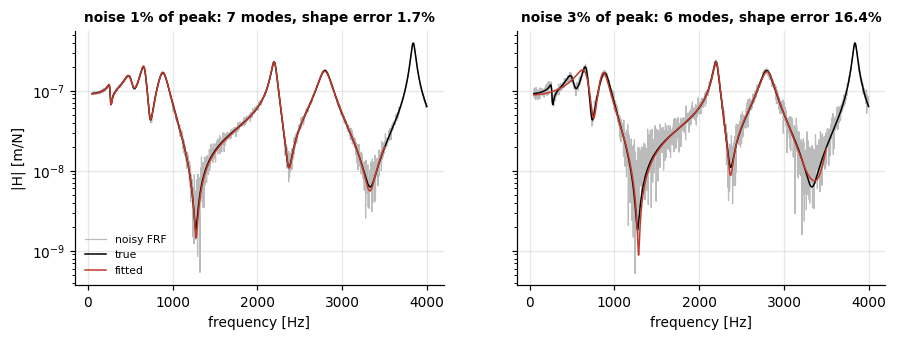
\includegraphics[width=0.95\linewidth]{figures/f_frf_fit.png}
\caption{FRF import on a synthetic transfer function with 1\% and 3\% noise: noisy input, true and fitted receptance magnitude.}\label{fig:frf}
\end{figure}

\subsection{Robustness to the operating regime}\label{sec:k10}
We repeated the gain calibration and the causal benchmark with the modal stiffness multiplied by 10, a regime in which the zero-order limit lies far above the cutting depth and the rms displacement is 5--8~$\mu$m (Table~\ref{tab:regime}). The effect-size calibration then needs gains 45 and 38 times larger ($g_\text{acc}=3.5\times10^{-4}$, $g_\text{mic}=0.43$ instead of $7.7\times10^{-6}$ and $0.0116$; the grid had to be extended to find them), confirming that the nominal gains compensate an amplitude mismatch. The soft-sensor errors are unchanged (log-factor RMSE $0.07$--$0.29$). Table~\ref{tab:k10} and Figure~\ref{fig:k10} show that the main finding persists: top-1 accuracy at $m{=}10$ is $0.53$--$0.98$ with a shared generator and falls to $0.32$--$0.62$ under shifted parameters (nominal: $0.52$--$0.98$ and $0.35$--$0.71$). The ordering of the algorithms is partly regime-dependent: BARO no longer collapses under shift ($0.50$ instead of $0.35$) and Smooth Traversal remains best ($0.62$). The graph ablation and the real-data comparisons were not repeated in this regime.
\begin{table}[t]\centering\small
\caption{Top-1 accuracy $\uparrow$ at $m{=}10$ (mean over 5 root causes) at nominal parameters and with the modal stiffness multiplied by 10; best per column in bold.}\label{tab:k10}
\begin{tabular}{lcccc}
\toprule
& \multicolumn{2}{c}{Nominal parameters (above stability limit)} & \multicolumn{2}{c}{Stiffness $\times10$ (stable regime)} \\
\cmidrule(lr){2-3}\cmidrule(lr){4-5}
Algorithm & Same generator & Shifted & Same generator & Shifted \\
\midrule
BRCD & 0.90 & 0.58 & 0.94 & 0.49 \\
RCD & 0.80 & 0.39 & 0.76 & 0.40 \\
RCG & 0.90 & 0.59 & 0.92 & 0.48 \\
Smooth Traversal & \cellcolor{gray!20}\textbf{0.98} & \cellcolor{gray!20}\textbf{0.71} & \cellcolor{gray!20}\textbf{0.98} & \cellcolor{gray!20}\textbf{0.62} \\
BARO & 0.94 & 0.35 & 0.94 & 0.50 \\
SimpleRCA & 0.52 & 0.44 & 0.53 & 0.32 \\
\midrule
Chance (1/14) & 0.07 & 0.07 & 0.07 & 0.07 \\
\bottomrule
\end{tabular}

\end{table}
\begin{figure}[t]\centering
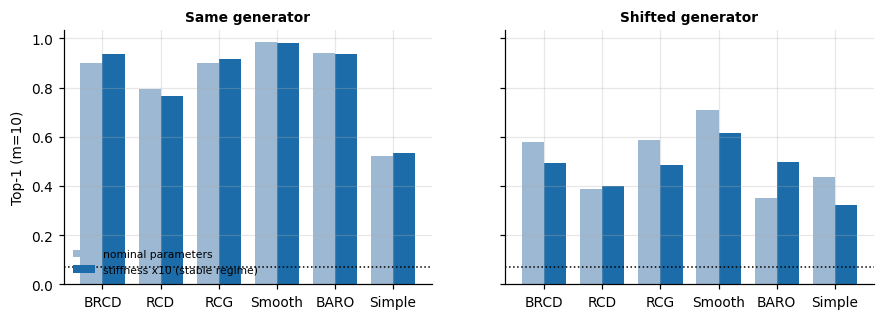
\includegraphics[width=0.95\linewidth]{figures/f_k10.png}
\caption{Robustness to the operating regime: top-1 at $m{=}10$ for nominal parameters and for a stiffer, stable-regime parameter set.}\label{fig:k10}
\end{figure}

\subsection{Planned evaluation on real multi-cause data (placeholder values)}\label{sec:planned}
Table~\ref{tab:planned} and Figure~\ref{fig:planned} show the layout of the central experiment of Section~\ref{sec:limits}. \fake{\textbf{All values are placeholders and are not results; no such data have been collected.}}
\begin{table}[t]\centering\small
\caption{\fake{PLACEHOLDER (not real data).} Leave-one-configuration-out evaluation on real multi-cause cuts: top-1 $\uparrow$ and expected calibration error (ECE) $\downarrow$ per training mode, $k{=}8$ real cuts.}\label{tab:planned}
\begin{tabular}{lcccc}\toprule
Training mode & Top-1 $\uparrow$ & Top-3 $\uparrow$ & Macro-F1 $\uparrow$ & ECE $\downarrow$\\\midrule
(a) simulation only ($k{=}0$) & \fake{0.46} & \fake{0.78} & \fake{0.41} & \fake{0.19}\\
(b) simulation + fine-tune ($k{=}8$) & \best{\fake{0.70}} & \best{\fake{0.93}} & \best{\fake{0.66}} & \best{\fake{0.08}}\\
(c) real only ($k{=}8$) & \fake{0.58} & \fake{0.84} & \fake{0.52} & \fake{0.14}\\
(d) real, other configurations, no simulation & \fake{0.52} & \fake{0.81} & \fake{0.47} & \fake{0.12}\\
(e) (d) + FRF-anchored simulation & \fake{0.66} & \fake{0.90} & \fake{0.61} & \fake{0.10}\\\bottomrule
\end{tabular}
\end{table}
\begin{figure}[t]\centering
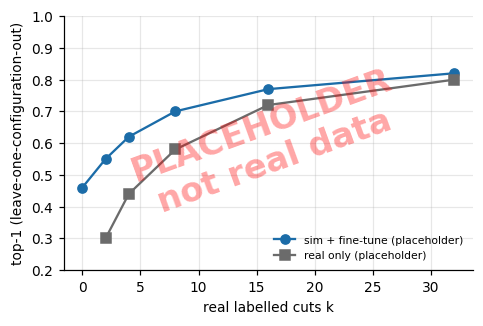
\includegraphics[width=0.5\linewidth]{figures/f_planned_kcurve.png}
\caption{\fake{PLACEHOLDER (not real data).} Planned learning curve: top-1 versus the number $k$ of real labelled cuts, with and without simulation pre-training.}\label{fig:planned}
\end{figure}

%% =============================================================================================
\section{Limitations and Next Steps}\label{sec:limits}
\paragraph{Scope limits.} Results are for one tool and material (MSM subset), one defective-tool comparison on a different tool, and force-only wear data (LUH). We have no real multi-cause data and therefore no validation of root-cause ranking on real cuts.
\paragraph{Open technical limits.} (i) The nominal simulator is above its stability limit at every real cutting condition and the fault gains absorb an amplitude mismatch of five orders of magnitude (Section~\ref{sec:regime}); (ii) the healthy baseline remains distinguishable from real data (balanced accuracy $0.82$--$0.95$ over the four variants); (iii) neither standard fault models nor a chipped-flute runout reproduce the defective-tool signature; (iv) the RCA algorithms are simplified re-implementations with unsourced constants, and the graph ablation depends on that choice; (v) the MSM microphone and accelerometer show a machine line near 1.5~kHz that contaminates the 1--3~kHz features; (vi) main causal tables use one split and seed, and only the ablation reports three seeds; (vii) fault severity ranges, gains, nominal physical parameters and the causal graph are assumptions; (viii) FRF import is tested only on synthetic transfer functions.
\paragraph{Planned evaluation on real multi-cause data.} The full collection and evaluation protocol is in \texttt{paper/DATA\_PROTOCOL.md}; the central test is leave-one-configuration-out over machine--tool--overhang configurations with measured FRFs, comparing real data only, FRF-anchored simulation only and their combination. We will collect cuts with designed causes (clamp stiffness, overhang, wear, depth or speed outside the stable range, imbalance, chipped flute) on at least two machines with hammer-test FRFs and force-coefficient calibration cuts, and evaluate by leave-one-machine-out and leave-one-configuration-out with: simulation only ($k{=}0$), simulation plus $k$ real samples, real only; top-1/top-3, macro-F1, calibration error and coverage--accuracy for an abstain option. Baselines: standard classifiers, domain-adversarial transfer \citep{wang2020datwear}, meta domain generalisation \citep{li2023metadg}, RMS and spectral-rule thresholds, FRF-based stability checks, and faithful implementations of the RCA algorithms. Decision gates: if the simulator with measured FRFs does not reproduce the measured stability boundary within an agreed tolerance, fix the model before collecting more; if no benefit at small $k$ appears, position the contribution as zero-shot ($k{=}0$), dataset and gap analysis.

\section{Conclusion}
We asked how far simulation can take root cause diagnosis in milling and measured it against real data in three places.
Simulated causal-RCA accuracy depends on how diagnostic nodes are built and falls from 0.80--0.98 to 0.35--0.71 under moderate generator mismatch, while the causal graph has no effect; the simulated healthy baseline and the signature of a real defective tool remain different from real data, and the nominal simulator operates above its stability limit; and on a public wear dataset simulation-only transfer is below a one-feature rule on two machines and brings no fine-tuning benefit, because the task is too easy to show one.
Simulation is necessary in principle for causes without real labels, but its value was not demonstrated on any real task we could test. These results define where simulation cannot yet be trusted and give a protocol to test it on real multi-cause data, which is the main limitation and the next step.

\section*{Availability}\label{sec:avail}
\begin{sloppypar}
\paragraph{Code.} \url{https://github.com/danghaidang04/RCA-for-Chatter-Simulation} (branch \texttt{cutting-sim-experiments}); \texttt{REPRODUCE.md} gives environment, data download, run order, seeds and expected outputs; every table and figure is generated from the result files by \texttt{paper/make\_tables.py} and \texttt{paper/make\_figures.py}. Licence: MIT \fake{(to be confirmed with the university)}. Archival DOI: \fake{to be assigned (Zenodo) at submission}.
\paragraph{Data.} MSM \citep{kim2026msm} (Kaggle, DOI 10.34740/kaggle/ds/8392825, CC BY 4.0) and LUH \citep{denkena2023luh} are obtained from their original sources and are not redistributed; derived features and all result files are in the repository.
\end{sloppypar}

\bibliographystyle{plainnat}
\bibliography{refs}

\appendix
\section{Parameter provenance}\label{app:registry}
\begin{table}[h]\centering\small
\caption{Every simulator parameter, its tier (fixed / range / learned / assumed) and verification status.}
\begin{tabular}{p{5.2cm}p{1.8cm}p{6.5cm}}
\toprule
Parameter & Tier & Verification \\
\midrule
tool diameter, flutes, flute length, overall length & FIXED & verified (read from catalog table p.5) \\
helix angle $\beta$ & FIXED & medium: from series feature list (p.3); not stated per part number \\
tool substrate/coating & FIXED & medium \\
N, ae, feed F, direction & FIXED & verified (N and F equal mtc Spindle\_Speed/Feed\_Rate, ratio 1.000) \\
axial depth ap = engaged depth & FIXED & assumption (not measured) \\
workpiece AA 6061; wet cutting (coolant flood) & FIXED & verified (stated in paper) \\
sampling: accelerometer 51.2 kHz, audio 48 kHz & FIXED & verified (stated in paper) \\
analysis window 0.3 s & FIXED & design choice \\
model structure: regenerative DDE, shear+edge force, ZOA lobes & FIXED & model structure \\
\midrule
Kt, Kr, Kte, Kre (AA 6061, this tool, wet) & LEARNED & NO usable source (rejected: steel-like values; dry-cutting AA6061 value unverified) \\
tool-tip FRF: fn\_x, fn\_y, $\zeta$, modal stiffness k & LEARNED & NO source for this tool/holder/stick-out (Altintas Ex.2 FRF rejected: different machine and tool) \\
spindle imbalance U & LEARNED & NO source (rotor mass, balance grade unknown) \\
sensor gains, noise floors, rpm-dependence & LEARNED & NO source (sensors uncalibrated: mic dBFS, accelerometer mm/s\^{}2) \\
runout; between-cut variability $\sigma$ (Kt, runout, roughness) & LEARNED & NO source \\
\midrule
chip-thickness cap 0.3 mm; roughness noise base 0.02 $\mu$m & ASSUMED & own assumption \\
\bottomrule
\end{tabular}

\end{table}

\section{Nominal simulator parameters}\label{app:simparams}
\begin{table}[h]\centering\small
\caption{Nominal values and numerical search bounds of the 16 simulator parameter groups (\texttt{cutting\_sim/model\_v4.py}). The bounds are numerical, not claims from the literature. Fixed quantities: 2 flutes, $D{=}6.35$~mm, $\beta{=}30^\circ$, $a_p{=}38.1$~mm, $N_z{=}8$, $\Delta t{=}1/25\,600$~s, $h_{\max}{=}0.3$~mm.}
\begin{tabular}{lccl}
\toprule
Parameter & Nominal & Unit & Numerical search bounds \\
\midrule
$g_{\mathrm{acc}}$ & 2.48e-03 & -- & 6.14e-06 to 7.39e+00 \\
acc. noise floor & 0.018 & g & 0.000 to 1.000 \\
$g_{\mathrm{mic}}$ & 1.00 & -- & 0.00 to 403.43 \\
mic. noise floor & 0.050 & Pa & 0.000 to 1.000 \\
natural freq.\ $f_x$ & 1500 & Hz & 500 to 4000 \\
natural freq.\ $f_y$ & 1500 & Hz & 500 to 4000 \\
damping ratio $\zeta$ & 0.030 & -- & 0.005 to 0.150 \\
modal stiffness $k$ & 3.0e+06 & N/m & 5.0e+05 to 2.0e+07 \\
tangential coeff.\ $K_t$ & 7.0e+08 & N/m$^2$ & 2.0e+08 to 2.0e+09 \\
ratio $K_r/K_t$ & 0.30 & -- & 0.10 to 1.50 \\
edge coeff.\ $K_{te}$ & 2.0e+04 & N/m & 1.0e+03 to 1.0e+05 \\
edge coeff.\ $K_{re}$ & 2.0e+04 & N/m & 1.0e+03 to 1.0e+05 \\
imbalance $U$ & 2.3e-06 & kg\,m & 2.1e-09 to 2.5e-03 \\
acc. noise rpm exponent & 1.0 & -- & -2.0 to 8.0 \\
mic. noise rpm exponent & 1.0 & -- & -2.0 to 8.0 \\
runout & 5.0 & $\mu$m & 1.0 to 30.0 \\
\bottomrule
\end{tabular}

\end{table}

\section{Methodological pitfalls found along the way}
\begin{enumerate}
\item Plain accuracy of a classifier two-sample test with unequal sizes has a chance level above 0.5; use balanced accuracy.
\item Real and simulated features must use windows of identical length; a 20-fold mismatch inflated variance threefold.
\item Out-of-sample residuals are needed to estimate between-cut variation when the regression can interpolate each cut.
\item Distribution matching alone did not identify the fault gain; effect-size matching was used.
\item Nodes trained on the generator's labels make a causal benchmark circular.
\item Force-axis sign conventions differ between machines; a signed mean force put zero-shot transfer below chance.
\item Plotting raw simulator output early would have exposed the stability problem of Section~\ref{sec:regime}; check the operating regime of a simulator against the stability limit before using it.
\end{enumerate}
\end{document}
